% 中山大学科技类及IT类实验报告文档类(LaTeX模板)
\documentclass{sysucseexp}
\usepackage{fontspec,inconsolata,url}
\setmainfont{Times New Roman}
\setmonofont{Consolas}

% 载入需要的宏包
\input{settings/packages.tex}
% 进行必要的设置
\input{settings/format.tex}
% 专用术语宏命令进行必要的设置
\input{settings/terms.tex}

% 设置封面基本信息
\sysucseset{
  college = {计算机学院},
  projname = {计算复杂性理论实验},
  title = {第二次编程作业},
  stunoleader = {23336150},
  authorleader = {刘昊},
  stunoone = {23336203},
  authorone = {任意嵘},
  stunotwo = {23336193},
  authortwo = {彭怡萱},
  major = {计算机科学与技术},
  adviser = {冯剑琳},
  startdate = {2026年4月X日},
  enddate = {4月X日}
}

\begin{document}

% 封面及目录
\makecover
\tableofcontents
\cleardoublepage
\pagestyle{main}

%%%%%%%%%%%%%%%%%%%%%%%%%%%%%%%%%%%%%%%%

\section{摘要}

% TODO: 简述实验目的和主要内容
本实验旨在实现NP完全性理论中的多项式时间归约算法，具体包括：

\begin{itemize}
    \item 任务1：实现3SAT问题到节点覆盖问题（Vertex Cover）的多项式时间归约
    \item 任务2：实现3SAT问题到独立集问题（Independent Set）的多项式时间归约
\end{itemize}

通过本实验，深入理解NP完全性理论、多项式时间归约的概念和方法，掌握如何证明问题的NP完全性。

\vspace{1em}
\textbf{关键词}：NP完全性、多项式时间归约、3SAT、节点覆盖、独立集

%%%%%%%%%%%%%%%%%%%%%%%%%%%%%%%%%%%%%%%%

\section{问题描述}

\subsection{3SAT问题定义}

% TODO: 填写3SAT问题的形式化定义
3SAT问题是布尔可满足性问题的一个重要子类。给定一个合取范式（CNF）形式的布尔公式$\phi$，其中每个子句恰好包含3个文字，判断是否存在一个真值赋值使得$\phi$为真。

\textbf{形式化定义}：

设$\phi = C_1 \land C_2 \land \cdots \land C_m$，其中每个子句$C_i = (l_{i1} \lor l_{i2} \lor l_{i3})$，$l_{ij}$为文字（变量$x_k$或其否定$\neg x_k$）。

\textbf{问题}：是否存在赋值$\sigma: \{x_1, \ldots, x_n\} \to \{0, 1\}$使得$\phi(\sigma) = 1$？

\subsection{节点覆盖问题定义}

% TODO: 填写节点覆盖问题的形式化定义
节点覆盖问题（Vertex Cover Problem）是一个经典的图论问题。

\textbf{形式化定义}：

给定无向图$G = (V, E)$和正整数$k$，判断是否存在$V$的子集$V' \subseteq V$，满足：
\begin{enumerate}
    \item $|V'| \leq k$
    \item 对于每条边$(u, v) \in E$，至少有一个端点在$V'$中（即$u \in V'$或$v \in V'$）
\end{enumerate}

\subsection{独立集问题定义}

% TODO: 填写独立集问题的形式化定义
独立集问题（Independent Set Problem）同样是图论中的经典问题。

\textbf{形式化定义}：

给定无向图$G = (V, E)$和正整数$k$，判断是否存在$V$的子集$V' \subseteq V$，满足：
\begin{enumerate}
    \item $|V'| \geq k$
    \item 对于任意两个顶点$u, v \in V'$，有$(u, v) \notin E$（即$V'$中的顶点两两不相邻）
\end{enumerate}

\subsection{归约关系}

% TODO: 说明归约的理论基础
本实验需要实现以下多项式时间归约：
\begin{itemize}
    \item $3SAT \leq_p VertexCover$
    \item $3SAT \leq_p IndependentSet$
\end{itemize}

这些归约证明了节点覆盖问题和独立集问题都是NP完全的。

%%%%%%%%%%%%%%%%%%%%%%%%%%%%%%%%%%%%%%%%

\section{算法设计}

% ==================== 任务1：人员B填写 ====================
\subsection{任务1：3SAT $\to$ 节点覆盖归约算法}
% TODO: 人员B填写本节全部内容

\subsubsection{归约思路}

% TODO: 人员B - 详细描述归约思路，参考课件pnp3.ppt
将3SAT实例$\phi$转换为图$G$和整数$k$，使得$\phi$可满足当且仅当$G$存在大小不超过$k$的节点覆盖。

\subsubsection{构造方法}

% TODO: 人员B - 描述图的构造方法，包括变量构件、子句构件、连接方式
\textbf{步骤1：变量构件}

对于每个变量$x_i$，构造一个变量构件（两个顶点相连的边）。

\textbf{步骤2：子句构件}

对于每个子句$C_j$，构造一个子句构件（三个顶点组成的三角形）。

\textbf{步骤3：连接构件}

将子句构件中的顶点与变量构件中的顶点相连。

\subsubsection{正确性证明}

% TODO: 人员B - 证明归约的正确性，需证明双向蕴含
证明：$\phi$可满足 $\Leftrightarrow$ $G$存在大小为$k$的节点覆盖。

% ==================== 任务2：人员C填写 ====================
\subsection{任务2：3SAT $\to$ 独立集归约算法}
% TODO: 人员C填写本节全部内容

\subsubsection{归约思路}

% TODO: 人员C - 详细描述归约思路，参考课件"Independent Set is NP-complete.pdf"
利用节点覆盖与独立集的补集关系，可以直接从任务1的结果导出独立集归约。

\subsubsection{构造方法}

% TODO: 人员C - 描述图的构造方法
可以复用任务1的构造，或采用其他构造方法。

\subsubsection{正确性证明}

% TODO: 人员C - 证明归约的正确性，需证明双向蕴含
证明：$\phi$可满足 $\Leftrightarrow$ $G$存在大小为$k$的独立集。

%%%%%%%%%%%%%%%%%%%%%%%%%%%%%%%%%%%%%%%%

\section{实现细节}

% ==================== 数据结构：人员A已实现，BC可参考 ====================
\subsection{数据结构设计}

\subsubsection{CNF公式表示}

% 已由人员A实现，详见 src/models/formula.py
\begin{lstlisting}[language=Python]
# 人员A已实现，位于 src/models/formula.py
class Literal:
    """表示一个文字（变量或其否定）"""
    variable: str      # 变量名
    negated: bool      # 是否取反
    
    def negate(self) -> Literal:
        """返回取反的文字"""
        return Literal(self.variable, not self.negated)

class Clause:
    """表示一个子句（3个文字的析取）"""
    literals: List[Literal]
    
    def get_variables(self) -> Set[str]:
        """获取子句中所有变量名"""
        return {lit.variable for lit in self.literals}

class Formula3SAT:
    """表示3SAT公式（多个子句的合取）"""
    clauses: List[Clause]
    variables: Set[str]  # 所有变量集合
    
    def get_clause_count(self) -> int:
        """获取子句数量"""
        return len(self.clauses)
\end{lstlisting}

\subsubsection{图的表示}

% 已由人员A实现，详见 src/models/graph.py
\begin{lstlisting}[language=Python]
# 人员A已实现，位于 src/models/graph.py
class Graph:
    """表示无向图"""
    def add_node(self, label: str = "") -> int:
        """添加节点，返回节点ID"""
        
    def add_edge(self, u: int, v: int) -> None:
        """添加无向边"""
        
    def nodes(self) -> List[int]:
        """获取所有节点ID"""
        
    def edges(self) -> List[Tuple[int, int]]:
        """获取所有边"""
        
    def get_label(self, node_id: int) -> str:
        """获取节点标签"""
        
    def is_vertex_cover(self, vertices: Set[int]) -> bool:
        """检查是否是顶点覆盖"""
        
    def is_independent_set(self, vertices: Set[int]) -> bool:
        """检查是否是独立集"""
        
    def to_networkx(self) -> nx.Graph:
        """转换为networkx图对象"""
\end{lstlisting}

\subsubsection{解析器模块}

% 已由人员A实现，详见 src/parsers/cnf_parser.py
\begin{lstlisting}[language=Python]
# 人员A已实现，位于 src/parsers/cnf_parser.py

# txt文件解析器（本次作业规定格式）
def parse_txt_file(file_path: str) -> Formula3SAT:
    """
    解析txt格式的3SAT公式文件
    格式：每行3个文字，空格分隔，-x表示否定
    """
    
# CNF字符串解析器（支持多种格式）
def parse_cnf_string(s: str) -> Formula3SAT:
    """
    支持格式：
    - 数学符号: "(x ∨ y ∨ ¬z) ∧ (¬x ∨ ¬y ∨ z)"
    - 编程格式: "(x|y|~z)&(~x|~y|z)"
    """
    
# DIMACS格式解析器
def parse_dimacs(file_path: str) -> Formula3SAT:
    """解析DIMACS CNF格式文件"""
\end{lstlisting}

\subsubsection{可视化模块}

% 已由人员A实现，详见 src/utils/visualization.py
\begin{lstlisting}[language=Python]
# 人员A已实现，位于 src/utils/visualization.py

def draw_reduction_graph_spec(formula_str, graph, k_or_n,
                              problem_type, output_path):
    """
    按规格说明要求绘制归约结果图：
    - 圆形节点，标签格式如 C2:¬x
    - 不同线型区分子句边和矛盾边
    - 包含问题文本描述
    """

def format_node_label(clause_index: int, literal_str: str) -> str:
    """格式化节点标签，如 C1:x 或 C2:¬x"""
\end{lstlisting}

\subsubsection{主程序入口}

% 已由人员A实现，详见 main.py
\begin{lstlisting}[language=Python]
# 人员A已实现，位于 main.py

# 命令行使用示例：
# python main.py --task 1 --input test/task1_course_example.txt
# python main.py --task 2 --input test/task2_course_example.txt
# python main.py --all  # 运行所有测试用例

def run_task1(input_file: str, output_dir: str):
    """运行任务1：3SAT到点覆盖的归约"""
    
def run_task2(input_file: str, output_dir: str):
    """运行任务2：3SAT到独立集的归约"""
\end{lstlisting}

% ==================== 任务1代码：人员B填写 ====================
\subsection{任务1关键代码说明}
% TODO: 人员B填写本节内容

\subsubsection{归约函数}

% TODO: 人员B - 实现并展示归约函数的关键代码
\begin{lstlisting}[language=Python]
# 人员B需实现，位于 src/reductions/vertex_cover.py
def reduce_3sat_to_vertex_cover(formula: Formula3SAT) -> Tuple[Graph, int]:
    """
    将3SAT实例归约为节点覆盖实例
    
    Args:
        formula: 3SAT公式
        
    Returns:
        (G, k): 图G和整数k，使得公式可满足 ⟺ G有大小为k的节点覆盖
    """
    # TODO: 人员B实现归约算法
    pass
\end{lstlisting}

\subsubsection{解的转换}

% TODO: 人员B - 实现从节点覆盖提取变量赋值的代码
\begin{lstlisting}[language=Python]
# TODO: 人员B实现
def extract_assignment_from_cover(cover: Set[int], formula: Formula3SAT) -> Dict[str, bool]:
    """
    从节点覆盖提取变量赋值
    
    Args:
        cover: 节点覆盖集合
        formula: 原始3SAT公式
        
    Returns:
        变量赋值字典 {变量名: True/False}
    """
    pass
\end{lstlisting}

% ==================== 任务2代码：人员C填写 ====================
\subsection{任务2关键代码说明}
% TODO: 人员C填写本节内容

\subsubsection{归约函数}

% TODO: 人员C - 实现并展示归约函数的关键代码
\begin{lstlisting}[language=Python]
# 人员C需实现，位于 src/reductions/independent_set.py
def reduce_3sat_to_independent_set(formula: Formula3SAT) -> Tuple[Graph, int]:
    """
    将3SAT实例归约为独立集实例
    
    Args:
        formula: 3SAT公式
        
    Returns:
        (G, n): 图G和整数n，使得公式可满足 ⟺ G有大小为n的独立集
    """
    # TODO: 人员C实现归约算法
    pass
\end{lstlisting}

\subsubsection{解的转换}

% TODO: 人员C - 实现从独立集提取变量赋值的代码
\begin{lstlisting}[language=Python]
# TODO: 人员C实现
def extract_assignment_from_indset(indset: Set[int], formula: Formula3SAT) -> Dict[str, bool]:
    """
    从独立集提取变量赋值
    
    Args:
        indset: 独立集
        formula: 原始3SAT公式
        
    Returns:
        变量赋值字典 {变量名: True/False}
    """
    pass
\end{lstlisting}

%%%%%%%%%%%%%%%%%%%%%%%%%%%%%%%%%%%%%%%%

\section{测试结果}

% ==================== 测试环境：人员A填写 ====================
\subsection{测试环境}

% 人员A填写
\begin{itemize}
    \item 操作系统：Windows 11 / Linux
    \item Python版本：3.8+
    \item 依赖库：networkx, matplotlib（用于可视化）
\end{itemize}

% ==================== 课件例子测试：人员B和C分别填写各自任务 ====================
\subsection{课件例子测试}

% 测试用例已定义在 tests/test_cases.py
% COURSE_EXAMPLE = "(x ∨ y ∨ ¬z) ∧ (¬x ∨ ¬y ∨ z) ∧ (¬x ∨ y ∨ ¬z)"

\subsubsection{任务1测试（人员B填写）}

% TODO: 人员B - 添加任务1的课件例子测试结果
\textbf{输入}：3SAT公式$\phi_1 = (x \lor y \lor \neg z) \land (\neg x \lor \neg y \lor z) \land (\neg x \lor y \lor \neg z)$

\textbf{归约结果}：
\begin{itemize}
    \item 图$G_1$：顶点数$|V| = $ TODO: 人员B填写，边数$|E| = $ TODO: 人员B填写
    \item 参数$k = $ TODO: 人员B填写
\end{itemize}

% TODO: 人员B - 添加归约结果图示
% \begin{figure}[H]
%     \centering
%     \includegraphics[width=0.8\textwidth]{figs/task1_course_example.png}
%     \caption{任务1课件例子归约结果}
%     \label{fig:task1_course_example}
% \end{figure}

\textbf{验证结果}：
% TODO: 人员B - 添加验证结果，说明归约的正确性

\subsubsection{任务2测试（人员C填写）}

% TODO: 人员C - 添加任务2的课件例子测试结果
\textbf{输入}：3SAT公式$\phi_1 = (x \lor y \lor \neg z) \land (\neg x \lor \neg y \lor z) \land (\neg x \lor y \lor \neg z)$

\textbf{归约结果}：
\begin{itemize}
    \item 图$G_1$：顶点数$|V| = $ TODO: 人员C填写，边数$|E| = $ TODO: 人员C填写
    \item 参数$n = $ TODO: 人员C填写
\end{itemize}

% TODO: 人员C - 添加归约结果图示
% \begin{figure}[H]
%     \centering
%     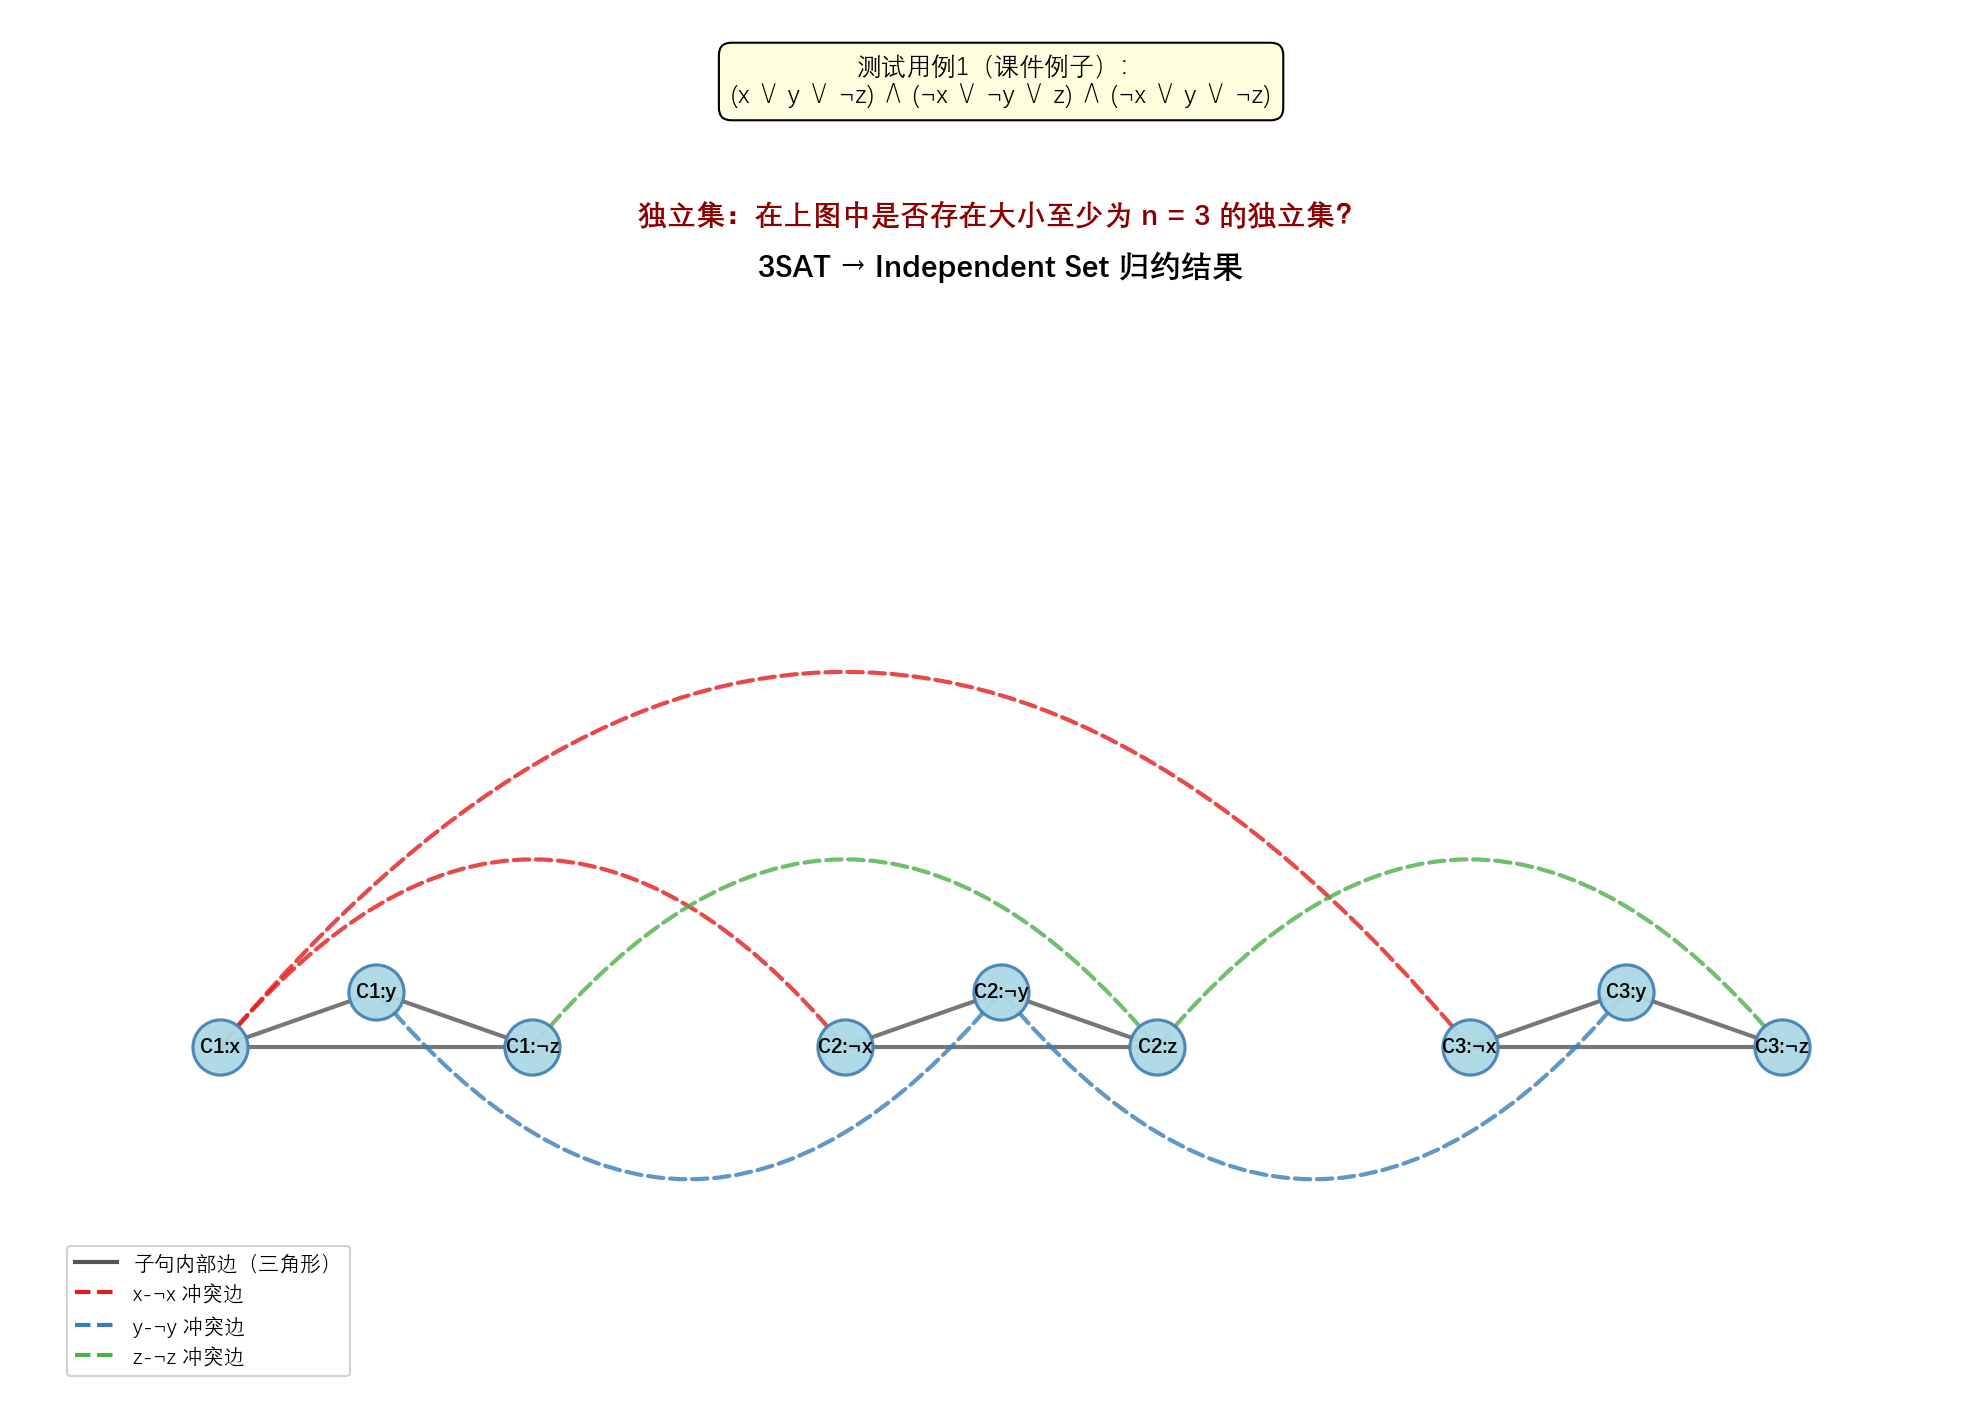
\includegraphics[width=0.8\textwidth]{figs/task2_course_example.png}
%     \caption{任务2课件例子归约结果}
%     \label{fig:task2_course_example}
% \end{figure}

\textbf{验证结果}：
% TODO: 人员C - 添加验证结果，说明归约的正确性

% ==================== 自定义例子测试：人员B和C分别填写 ====================
\subsection{自定义例子测试}

% 测试用例已定义在 tests/test_cases.py
% CUSTOM_EXAMPLE = "(x ∨ y ∨ ¬z) ∧ (¬x ∨ z ∨ w) ∧ (y ∨ ¬w ∨ u) ∧ (¬y ∨ ¬u ∨ x) ∧ (z ∨ w ∨ ¬u) ∧ (¬x ∨ ¬z ∨ u)"

\subsubsection{任务1测试（人员B填写）}

% TODO: 人员B - 添加任务1的自定义例子测试结果
\textbf{输入}：3SAT公式$\phi_2 = $ 6个子句的自定义公式

\textbf{归约结果}：
% TODO: 人员B填写

\textbf{验证结果}：
% TODO: 人员B填写

\subsubsection{任务2测试（人员C填写）}

% TODO: 人员C - 添加任务2的自定义例子测试结果
\textbf{输入}：3SAT公式$\phi_2 = $ 6个子句的自定义公式

\textbf{归约结果}：
% TODO: 人员C填写

\textbf{验证结果}：
% TODO: 人员C填写

% ==================== 结果分析：人员B和C共同填写 ====================
\subsection{结果分析}

% TODO: 人员B和C - 分析测试结果
\begin{itemize}
    \item 归约的正确性验证：TODO: 说明如何验证归约的正确性
    \item 时间复杂度分析：TODO: 分析归约算法的时间复杂度
    \item 空间复杂度分析：TODO: 分析归约算法的空间复杂度
\end{itemize}

%%%%%%%%%%%%%%%%%%%%%%%%%%%%%%%%%%%%%%%%

\section{结论与讨论}

% ==================== 实验总结：人员A填写总体框架，BC补充各自任务成果 ====================
\subsection{实验总结}

% 人员A填写总体框架，人员B和C补充各自任务的成果
本实验成功实现了3SAT问题到节点覆盖问题和独立集问题的多项式时间归约算法。主要成果包括：

\begin{enumerate}
    \item \textbf{公共模块}（人员A）：实现了CNF公式的解析和表示、图数据结构的设计
    \item \textbf{任务1}（人员B）：实现了3SAT到Vertex Cover的归约 % TODO: 人员B补充具体成果
    \item \textbf{任务2}（人员C）：实现了3SAT到Independent Set的归约 % TODO: 人员C补充具体成果
    \item 验证了归约的正确性
\end{enumerate}

% ==================== 遇到的问题：人员B和C分别填写各自遇到的问题 ====================
\subsection{遇到的问题和解决方案}

% TODO: 人员B填写任务1遇到的问题
\textbf{任务1（人员B）}：
\begin{itemize}
    \item 问题1：TODO: 人员B填写遇到的问题
    \begin{itemize}
        \item 解决方案：TODO: 人员B填写解决方案
    \end{itemize}
    \item 问题2：TODO: 人员B填写遇到的问题
    \begin{itemize}
        \item 解决方案：TODO: 人员B填写解决方案
    \end{itemize}
\end{itemize}

% TODO: 人员C填写任务2遇到的问题
\textbf{任务2（人员C）}：
\begin{itemize}
    \item 问题1：TODO: 人员C填写遇到的问题
    \begin{itemize}
        \item 解决方案：TODO: 人员C填写解决方案
    \end{itemize}
    \item 问题2：TODO: 人员C填写遇到的问题
    \begin{itemize}
        \item 解决方案：TODO: 人员C填写解决方案
    \end{itemize}
\end{itemize}

% ==================== 心得体会：三人各自填写 ====================
\subsection{心得体会}

% TODO: 人员A填写心得体会
\textbf{人员A}：通过本次实验，我深入理解了NP完全性理论中多项式时间归约的概念，掌握了如何设计公共数据结构为团队协作提供便利。...

% TODO: 人员B填写心得体会
\textbf{人员B}：TODO: 人员B填写心得体会，关于3SAT到节点覆盖归约的理解...

% TODO: 人员C填写心得体会
\textbf{人员C}：TODO: 人员C填写心得体会，关于3SAT到独立集归约的理解...

%%%%%%%%%%%%%%%%%%%%%%%%%%%%%%%%%%%%%%%%

\newpage

% ==================== 参考文献 ====================
\begin{thebibliography}{99}
    \bibitem{ref1}Sipser, M. (2012). \textit{Introduction to the Theory of Computation}. Cengage Learning.
    \bibitem{ref2}Garey, M. R., \& Johnson, D. S. (1979). \textit{Computers and Intractability: A Guide to the Theory of NP-Completeness}. W. H. Freeman.
    \bibitem{ref3}课程课件 pnp3.ppt
\end{thebibliography}

\end{document}